\documentclass[../eva1_scion.tex]{subfiles}
\begin{document}
    \chapter{Results}
    \section{Isolation Domains}
    SCION borrows basic ideas from the Border Gateway Protocol (BGP) like the idea of an Autonomous System (AS) which, like in BGP, repesents the smalest organisational unit. However, SCION introduces an additonal organisational unit called the Isolation Domain (ISD). The structure of an indivual ISD is ilustrated in \ref{fig:isd}a. An ISD is comprised of multiple core ASes, form logical unit whos members share a common set of resources and mutualy trust each other. As their name states, ISDs are intended to be selfsuficient units, the internal state of which must not leak out into other ISDs. \cite{scion_2011} While an arbitrary AS can be a member of an arbitrary ISD, or even multiple ISDs, it is expected that ISDs will form along shared comercial interests, legal juristiction or other political borders. \cite{scion_2017}.

    \subsection{IDS structure}
    As shown in ilustration \ref{fig:isd}a the main structure of an IDS is an undirected graph formed by a set of core ASes in the ISD core, client ASes and biderectional links between individual ASes. ASes may be connected by multiple redundant links. Although a link always carries biderctional traffic, there is an implied top down hirarchy of providers and consumers between the tiers in the graph. As in BGP a pair of ASes may enter an peering agreement, which is ilustrated is a dashed line. Links are also called path segments.

    \begin{figure}[ht]
        \centering
        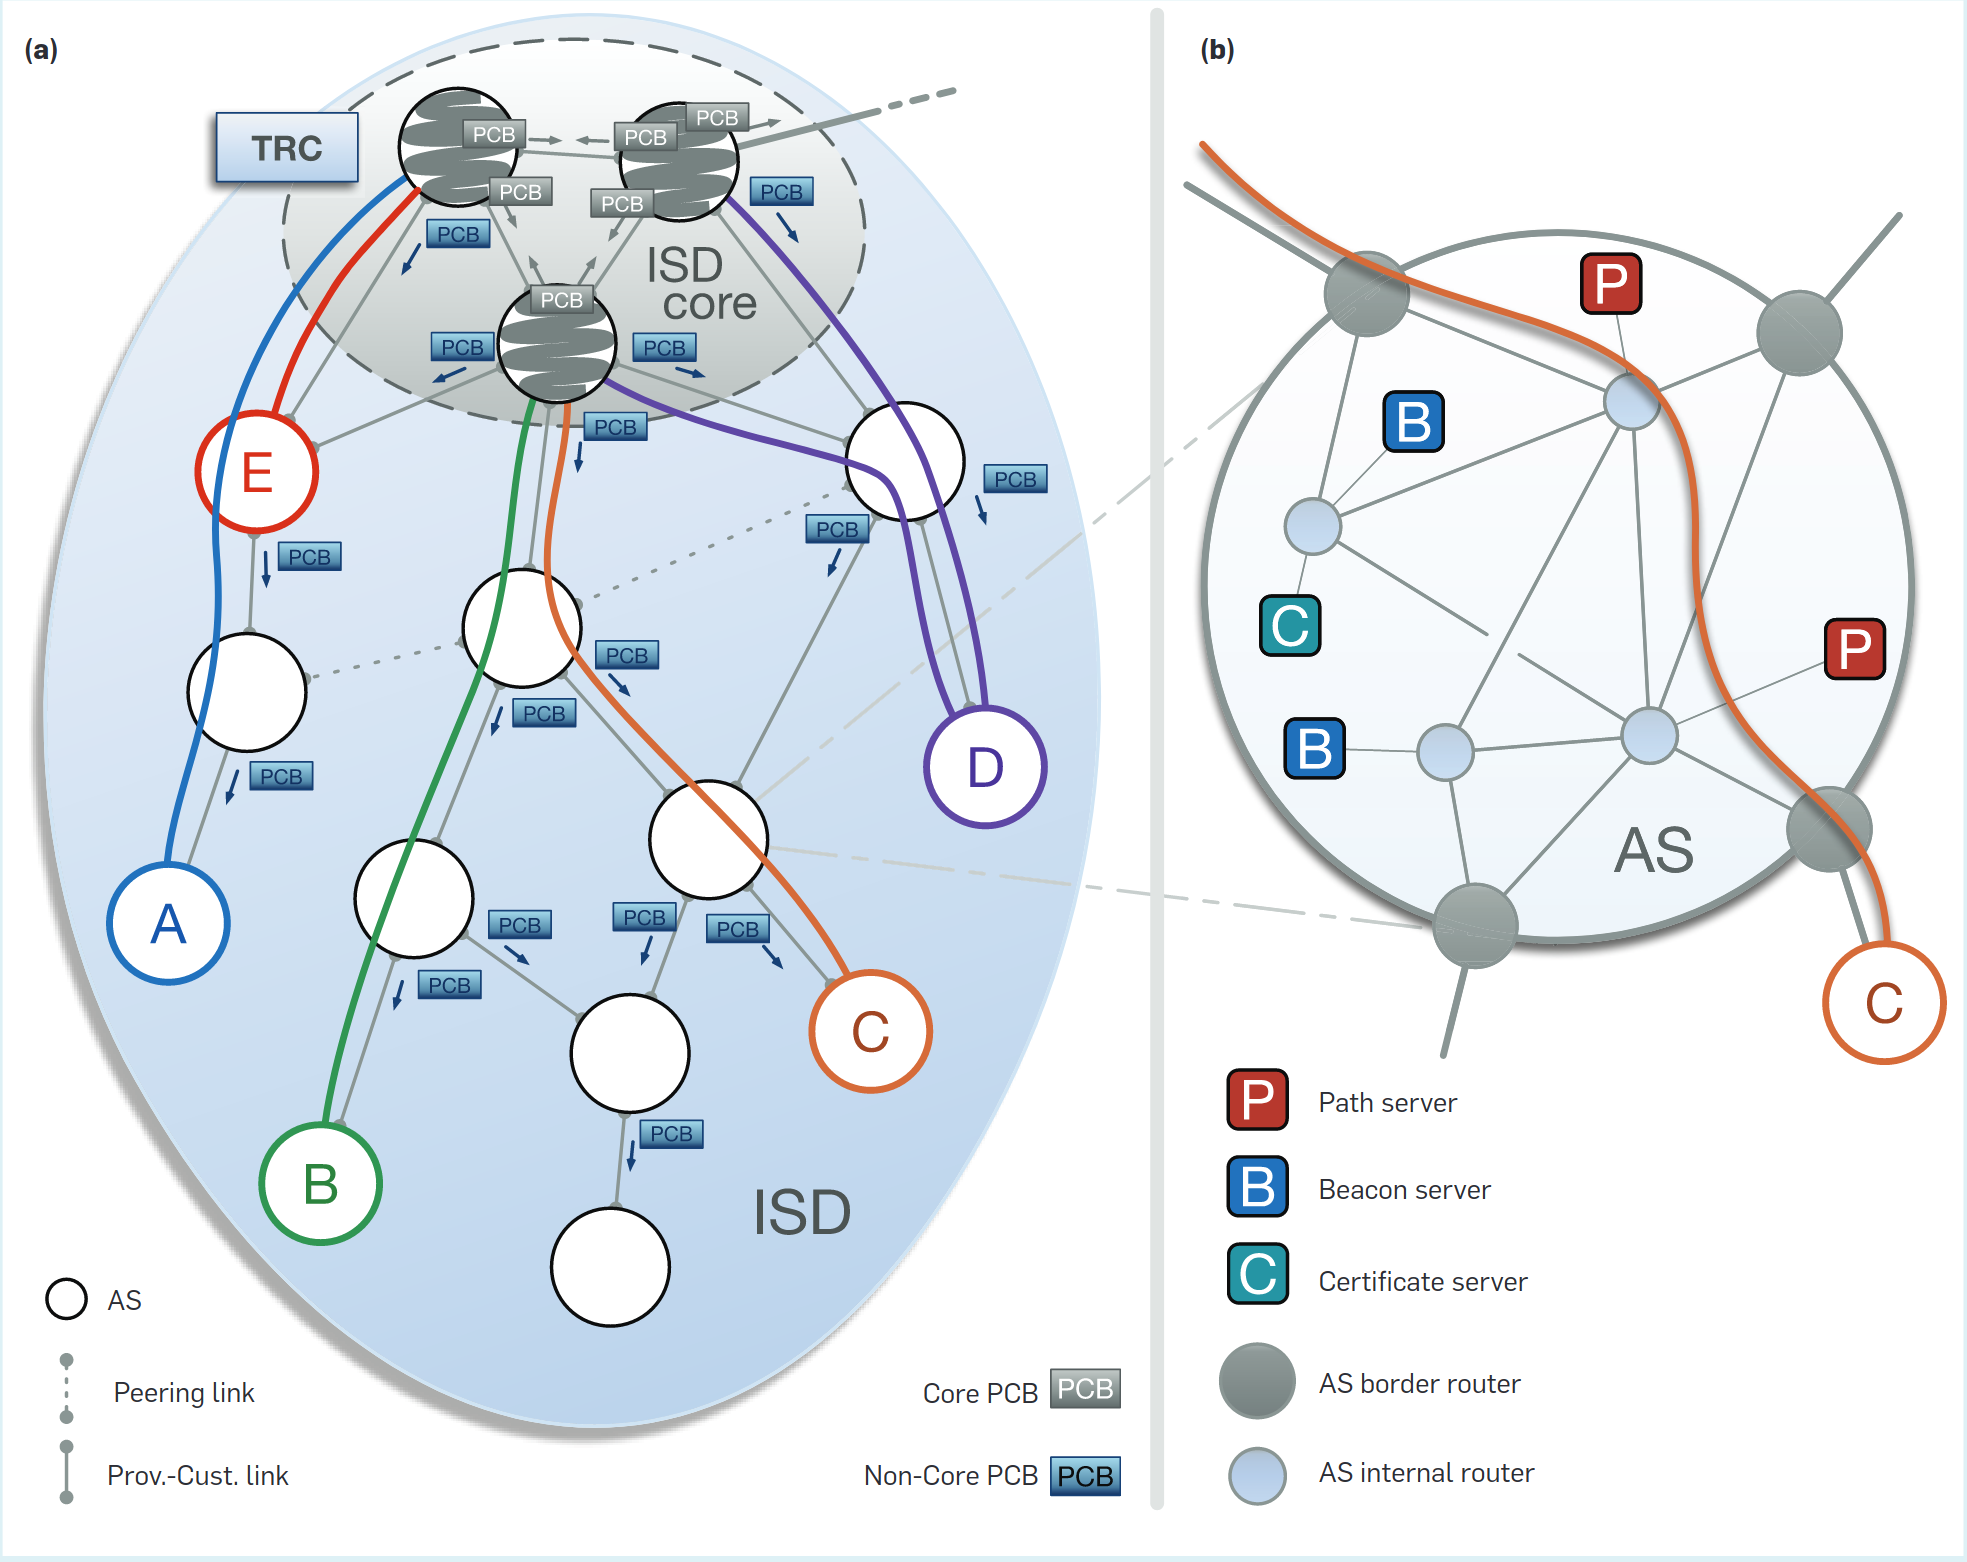
\includegraphics[width=0.8\linewidth]{scion_isd.png}
        \caption{Internal structure of an ISD. From \cite{scion_2017}}%
        \label{fig:isd}
    \end{figure}

    \subsection{AS and ISD Componants}
    In the following we will explore the componantes which are required to run an SCION AS and by extension a ISD since a single core AS is sufficient to form an IDS.

    SCION ASes look similar too their BGP cousins so fare as that they have internal routers and border routers and a set of routes through the AS. These ensure connectivity inside the AS and to neighbouring ASes. Border routers must be SCION enabled and must addhere to the common rules agreed upon inside the ISD, however each AS is free to choos its internal structure. In addition each AS needs at least a beacon server, a certificate server and a path server. Beacon servers are responbsible for path discovery and are required for beaconing process described in section \ref{ssec:beaconing}. Path server are repsonsible for caching and disimination of path information. They are involved in path resolution and assembly discussed in section \ref{ssec:path_assembly}. As SCION makes extensive us of certificates to validate paths and intities, certificate servers are deployed to cache and provide certificates in an AS.
    
    A core AS differs from other ASes in serveral important aspects. First of all core ASes have border routers which are connected to cores ASes in neighbouring. The beacon servers in the core ASes also take part in inter IDS beaconing (see section \ref{ssec:beaconing}), thus their path servers also hold path information on how to reach neighbouring ASes. Further more the ISD core is responsible for maintaining the trust root configuration (TRC).

    The trust root configuration (TRC) is policy which governs the operations of an ISD. The TRC lists the trust roots used in an ISD and thus is the central anchor of trust in an IDS. It is negotiated between the members of the ISD core and all ASes whishing to join an ISD need to accept the TRC. Neighbouring ISDs acknowledge an ISDs TRC by signing it. This makes ASes communicting across ISD bordes able to trust signatures originating from an neighouring ISD. Each TRC also holds a number of policies on how the TRC is used. Modifications to the TRC are only possible of multiple core ASes signe updated TRC, which prevents a rouge core AS from corupting the TRC. The number of required signatures for different kinds of changes is governed by the policies encoded in the TRC.

    Until now we looked at the static componants which make up an ISD, however the real world internet is not a static thing, so an ISD isn't either. To better manage complexity SCION is devided into a controll plane and a data plane. The control plane is concerned with discovering and maintaining paths, while the data plane uses these paths in the processes of path assembly and packet fowarding.

    \section{Control Plane}
    As mentioned above SCION has taken inspiration form BGP and the paths discovery is an other place where this is evident. SCION uses an beaconing process to discover all available paths and disiminate certain information inside an ISDs.  These beacons are called patch-segment construction beacons (PCBS) and are  sent from beacon servers in the ISD core t travle down the ISD graph as an policy constrained multipath flood. \cite{scion_2011}.

    \subsection{Path Discovery by Beaconing}\label{ssec:beaconing}
    Initialy the path server in a core ISD issues a PCB containing only the exit interface it originates from. A path server in a neighbouring AS receiving an incomming will forward it to all its client ASes. Befor forwarding the PCB it creates a  record of the ingress inteface, egress interface and available peers and appends it to the PCB. Each of these entries in path is protected my a MAC. While the PCB is cryptographically signed before it is sent out. In this way a PCB accumulates verifyable path information as a so called path-segment while it is forwarded through the ISD. The information received in PCBs is cached in the local path servers, so end hosts in an ISD have a way to look up path information. Important to note is that PCBs are not sent out through peering links as this would lead douplicate paths or might lead to intra-ISD beacons leaking into other ISDs.

    PCBs traveling down collect what are called down paths, but since all paths forward packets bidirectionally, each down-segment can be converted into an up-segment by inverting the order or traversed ASes. Once an AS has received a number of path segments it can register some of them as down-paths segmemts with the core path servers. This has two important consequences:  An AS always knows how to reach its ISD core by creating recoding path segments from PCBs, however for a local path server to optain down-paths to other ASes it needs to query the a path server in the core. This gives each AS the unique ability to control by which paths it would whishes to be reached.

    When selecting down-paths an AS tries to select as diverse paths as possible in order reach maximum reduncy. This makes SCION an ineherently multipathed system. Apart from diversity, ASes can select for many different quality measure in their paths like low latency or anonymous forwarding

    \section{Data Plane}
    While the control plane deals with path discovery, the data plane deals with forwarding data. For this the data plane uses the path information supplied by the control plane to assemble paths.

    \subsection{Packet Carried Forwarding State}
    In SCION information need for routing a given package is stored in the packet itselfs. This is refered to as package carried forwarding state (PCFS) and several interessting properties of SCION a derived from this. A packet at least contains a path, since source and destination adresses are optional, if the path is unambigous in its contetxt. Consequently, during forwarding, a router reads only the path information, in order to forward the packet to the next AS. Since all routing information is carried by the packet, the need for routing tables is completly eliminated. The split into a locator (the path) and an identifier (the destination address), facilitates another interessting feature of: Only the destanation AS needs to be able to interpret the destination address. This allows each AS to choos its own addressing schema. This means that e.g IPv4 and IPv6 hosts can talk directly to each other using scion.

    The absence of routing tables simplyfies the routings process and thus allows the construction of simpler and more energy efficient machines. XY have observed a gain of xx  energy efficiency compared to traditional BGP routing. Thanks to hardware accelration of cryptographic opertions through technologies like Intel AES-NI, forwarding descissions in SCION become faster than in BGP. All a router needs to do is checking the validity of the path recorded in the packet and read the exit interface from it. If hardware acceleration is available the signature validition is so efficient, it out performs DRAM look-ups a BGP router needs to performe to reach its routing decission. 

    \subsection{Path Combination} \label{ssec:path_assembly}
    Path combination is the process performed by an end host to obtain valid before sending a packet. Up three path-segments are combined into an end-to-end path. First of all tho end host looks up the AS and address of the destination with a name server. Then it queries a path server for a path to this destination. After look-up one of five scenarios will play out:
    \begin{itemize}
        \item \textbf{On path} (as shown in figure \ref{fig:isd}a $A \rightarrow E$) the destination lies directly on the up-path to the ISD core.
        \item \textbf{Direct combination} (as shown in figure \ref{fig:isd}a $B \rightarrow D$) The path can be constructed by chaning a complete up-segment with a down segment. The up- and down-segment intersect in a core AS.
        \item \textbf{AS shortcut} (as shown in figure \ref{fig:isd}a $B \rightarrow C$) This scenario is similar to the direct combination but the destination lies on down-segment which intersects the up-segment in a none core AS on the way to the ISD core.The unused segments up to the ISD cor and back down are cut off.
        \item \textbf{Core path combination} (as shown in fuger \ref{fig:isd}a $A \rightarrow D$) A up and down path do not intersect at any point and need to be connected by a core path. This can either be an intra ISD or inter ISD path. This is one of two ways of traversing ISD borders.
        \item \textbf{Peering shortcut} (as shown in fuger \ref{fig:isd}a $A \rightarrow B$) The up-segment and the down segment are connected by a peering link, such that the peering link alows a shortcut to the destination. Analogous to the AS shortcut in this case the extranous path segments are discarded as well. Note that this type of shortcut can also traverse ISD borders.
    \end{itemize}

    Once the host has constructed a path it is encoded as PCFS in the packet header. The destination host can either take the path contained it the received packet and simply reverse it, or performe its own lookup and combination process. Of course this process is assisted by varous cashing mechanisms 
    \section{Trust Management}
    As stated in the introduction trust management is a hard problem to solve and SCION takes a few important steps towords solving this problem. First of all the architecture limits the scope of trust to a smaler set of trustees by introducing ISDs, secondly it reduces the number of trust roots to a managable number. This makes key revocatio, or certificate revocation respectively, much easier, since there is no need for every single end host on the whole internet needs to be informed indivdually. SCION also makes extensive use of trust transitivity offered by digital signatures. 

    \subsection{Trust agility}
    Trust agility is the concept that trust can be quickly if a key is compromised. This requires simple and quick key revocation. SCION enables this by effectively avoiding two secnerios:

    \begin{itemize}
        \item \textbf{Trust monopoly}: All the entities on the internet need to trust one root of trust, like in DNSSEC or BGP Sec. This scenario suffers from having a single point of failure and revoking a key in this system is going to create an adminstrative nightmare that affects the whole infrastructure.
        \item  \textbf{Trust oligopoly}: In this scenario there is a multitude of equally trusted roots of trust. An expmle for this is todays TLS PKI system. This scenario suffers from the fact that it exposes many points of failure and revoking keys is made dificult by the sheer amount of keys to manage.
    \end{itemize}

    This is achivied by introducing a hirarchy of trust. ASes use a number of different keys for different purposes and can replace the keys and employed algorithms autonomously, however the used keys always require a signature by a trust root. This enables neighbouring ASes and end host in different ASes or ISDs to check the validity of the keys and by extensions the data processed by these keys.

    In SCION trust is rooted in a small number of trust roots which are encoded in each ISDs TRC. This TRC is only valid inside the ISD it applies to, thus limiting the scope of trust to one ISD. Since linked ISDs signe each others TRCs trust is conveyed, by the transitive properties of trust, between ISDs. If an ISD revokes a trust roots key, all keys signed with it, become invalid at once. This change propagates quickly through the ISD own ASes as well as to neighbouring ISDs. From this a interessting property emerges: As long as there is a path available to a given resource, the path can always be validate.

    \section{SCION Adoption}
    SCION is designed with easy adoption in mind and offeres a number of attractive benefits to adopters. Designe elements such as the use of existing ASes and isolating the inner structure of an AS from the SCION architecture are specifically targeted at easy adopotion of SCION. For an AS to adopt SCION it needs to deploy border routes which are SCION capable, as well as deploying name, beacon, certificate and path servers. All these can run on comodity hardware or on existing routers and the rest of the AS can remain largely unchanged.

    Since 2017  a realworld SCION testbed is operational \ref{testbed_2017} which includes several high profile members such as Swisscom and Switch, as well as other financial like SIX and the Swiss National Bank \ref{snb} and acedemic institutions.

\end{document}
